\chapter{Literature Review}

Action recognition, a pivotal task in computer vision, involves identifying and categorizing human actions from video or image sequences. As a fundamental component in various applications, such as surveillance, human-computer interaction, and autonomous systems, action recognition has garnered substantial research attention. The history of action recognition traces back to early works focused on handcrafted features and shallow classifiers. Pioneering studies, such as those by \cite{laptev2008learning} and \cite{wang2009evaluation}, explored the extraction of local spatiotemporal features and their aggregation using bag-of-words or temporal pyramids. These methods, although significant at the time, were limited in their ability to capture complex and dynamic human actions.

With the advent of deep learning, action recognition witnessed a paradigm shift, achieving remarkable performance improvements. Convolutional Neural Networks (CNNs) emerged as a dominant approach in image-based action recognition. Notable works by \cite{simonyan2014very} with Two-Stream CNNs and \cite{carreira2017quo} using 3D CNNs played a pivotal role in driving this progress. These methods effectively learned hierarchical representations from raw pixel inputs, enabling more accurate recognition of complex actions.

Beyond RGB data, researchers explored the potential of skeleton data for action recognition. Skeleton-based action recognition, popularized by \cite{du2015skeleton}, represents human movements as a set of joint coordinates, capturing the underlying structural and temporal information. Techniques such as Graph Convolutional Networks (GCNs) introduced by \cite{yan2018spatial} further leveraged the graph structure of human skeletons for enhanced representation learning.

Moreover, the exploration of self-supervised learning in action recognition gained traction, addressing the challenges of data annotation and scalability. Works by \cite{misra2020self} demonstrated the effectiveness of pretext tasks, such as predicting temporal order or solving jigsaw puzzles, in learning meaningful representations from unannotated data.

In this literature review, we survey the key advancements in action recognition by briefly going through the literature of action recognition with RGB modality and then we will focus on skeleton data modality. We investigate historical progress, influential methodologies, and the transition toward deep learning. Additionally, we examine foundational works in skeleton-based action recognition, emphasizing the role of graph-based and attention mechanism-based approaches. Furthermore, we explore the emergence of self-supervised learning in the context of action recognition, highlighting its potential to alleviate data annotation challenges and facilitate scalable learning. By synthesizing and analyzing these works, we lay the groundwork for proposing a contrastive self-supervised learning approach for action recognition on 3D human skeleton data in the subsequent chapters of this master thesis.

\section{Action Recognition with RGB Data}
A key challenge in computer vision is action recognition using RGB data, which includes identifying and categorizing human activities from video sequences represented by red, green, and blue color channels. RGB data is captured using conventional cameras, making it readily available and widely used in various real-world applications. The introduction of RGB action recognition datasets has been instrumental in advancing the field. One of the pioneering datasets in this domain is the "UCF101" dataset introduced by \cite{soomro2012ucf101}. It comprises 101 action classes, covering diverse activities, and has played a vital role in benchmarking RGB action recognition methods. Another well-known dataset, the "HMDB51" dataset by \cite{kuehne2011hmdb}, contains 51 action classes and serves as another widely used benchmark for RGB action recognition.


Several recent research papers have made significant contributions to the field. For instance, \cite{tran2015learning} proposed the "Two-Stream Convolutional Networks" that integrated spatial and temporal streams to capture static appearance and motion information, respectively. This work demonstrated the efficacy of fusing RGB data with optical flow information for action recognition, achieving state-of-the-art performance on benchmark datasets. Furthermore, the introduction of "3D Convolutional Neural Networks" (C3D) by \cite{ji20123d} revolutionized the field. C3D leverages 3D convolutions to capture spatio-temporal patterns directly from RGB videos, demonstrating superior performance in action recognition compared to traditional 2D CNNs.

Since the introduction of I3D \cite{carreira2017quo}, 3D-CNN has emerged as the standard method for action recognition. Since then, the action recognition community has put out several cutting-edge 3D-CNN designs as \cite{feichtenhofer2020x3d}, \cite{feichtenhofer2019slowfast} that exceed I3D in accuracy and efficiency, as architectures examples shown in ~\ref{fig:3DConvNet}.

\begin{figure}
	\centering
	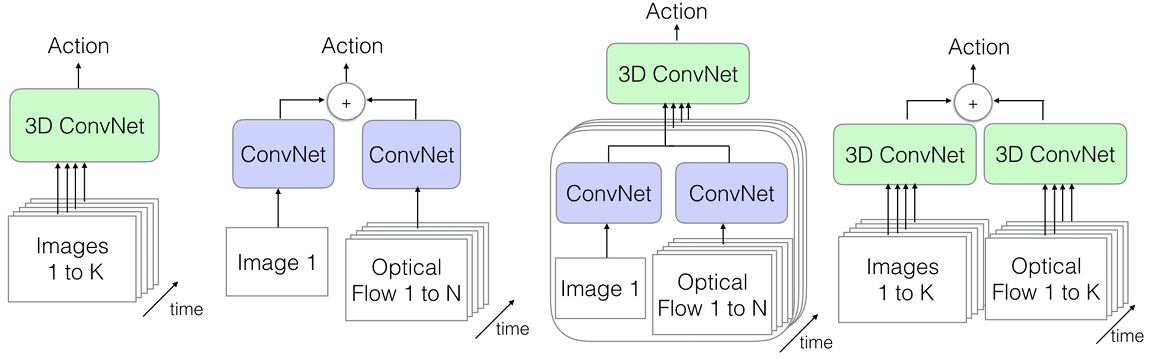
\includegraphics[width=.8\linewidth]{img/3DConvNet_approaches.JPG}
	\caption{Example from of previous RGB action recognition architectures, source from \cite{carreira2017quo}. (a) 3D-ConvNet. (b) Two-Stream. (c) 3D-Fused Two Stream. (d) Two-Stream 3D-ConvNet. K stands for the total number of frames in a video, whereas N stands for a subset of neighboring frames of the video.}\label{fig:3DConvNet}
\end{figure}


Moreover, several recent approaches have explored multi-modal fusion for enhanced action recognition. Methods combining RGB data with depth information or pose estimations have shown improved performance. For instance, \cite{franco2020multimodal}, \cite{tran2015learning} proposed a novel activity encoding method using temporal images from RGB video sequences and the integration of complementary information from a skeleton and temporal data. The proposed method outperforms state-of-the-art methods on public datasets. The challenges addressed in this paper include the difficulty of recognizing complex activities with high intra-class variability and the need for robustness to occlusions and noise. These challenges were addressed by using a multimodal approach that combines RGB and skeleton data, as well as a novel activity encoding method that uses temporal images. The limitations of this paper include the use of only two modalities (RGB and skeleton data) and the focus on recognizing activities in controlled environments. The proposed method may not generalize well to real-world scenarios with more complex backgrounds and lighting conditions.

RGB-based action recognition has witnessed remarkable progress, fueled by influential datasets and research papers. Despite these advancements, RGB-based action recognition still faces challenges. One major limitation is significant computational costs, making them less suitable for resource-constrained environments. However, ongoing research in the field aims to explore more efficient ways to handle large-scale labeled data and further improve the accuracy and robustness of RGB-based action recognition models.

With the advancements in pose estimation algorithms and models, annotating human pose estimation data with respective actions on a large scale has become more feasible. The availability of datasets containing 2D and 3D human skeleton information has significantly facilitated action recognition research. Human skeleton data provides a powerful representation that captures the essential structural and temporal information of actions while being resilient to environmental variations and occlusions. As a result, researchers have increasingly turned their attention to studying action recognition based on human skeletons. The benefits offered by skeleton-based action recognition methods, including improved robustness, reduced computational complexity, and better generalization across diverse scenarios, have led to a convergence of research efforts in this direction. In the next section, we will delve deeper into the advantages of using human skeleton representations for action recognition and explore the latest developments and methodologies in this rapidly evolving field.

\section{Action Recognition with Skeleton Data}
Action recognition with skeleton data is a crucial task in computer vision that involves identifying and categorizing human actions based on skeletal joint positions and temporal dynamics. Skeleton data is typically captured using depth sensors, motion capture systems, or pose estimation algorithms. Recent research has shown an increasing interest in skeleton-based action recognition due to its distinct advantages over other modalities, such as RGB data and depth sensors.

Skeleton data offers a compact and informative representation of human actions, focusing on the spatial arrangement and temporal dynamics of joints. Unlike RGB data, which requires complex processing to handle appearance changes and occlusions, skeleton data is inherently resilient to environmental variations, providing a robust representation for action recognition tasks. Additionally, compared to depth sensors, which can be sensitive to lighting conditions and limited in accuracy, skeleton data offers more precise and reliable joint information. One of the early skeleton action recognition datasets is the "NTU RGB+D" dataset introduced by \cite{shahroudy2016ntu}. This dataset contains 3D skeleton data captured by depth sensors, covering a diverse range of action classes and complex scenarios. Another notable dataset, the "Kinetics-Skeleton" dataset by \cite{kay2017kinetics}, provides 2D skeleton data extracted from videos in the Kinetics dataset, enabling a large-scale evaluation of skeleton-based action recognition models. Before the advent of deep learning, early methods of action recognition with skeleton data primarily relied on handcrafted features and traditional machine learning algorithms. These methods focused on extracting relevant information from the skeletal joint positions and designing effective classifiers to recognize actions. Major contributions during this era included the introduction of effective feature descriptors and the design of efficient classifiers.

One of the early approaches involved the use of histograms of joint angles or velocities as feature representations (e.g.,\cite{xia2012view}). By quantizing joint angles or velocities into bins and constructing histograms, these methods attempted to capture the spatial and temporal dynamics of actions. \cite{blank2005actions} is another approach involved the representation of actions as sequences of key poses or motion primitives. These key poses were identified based on keyframes or important points in the action sequences, providing a concise representation for recognition. Early methods also explored the application of traditional machine learning algorithms, such as Support Vector Machines (SVMs) and Hidden Markov Models (HMMs), to classify actions based on handcrafted features. These classifiers aimed to learn discriminative patterns from the extracted features and make predictions on new unseen sequences. However, these early methods had several limitations. Handcrafted feature engineering required domain expertise and manual design, making the process labor-intensive and potentially limiting the representation power of the features. Furthermore, these approaches struggled to successfully capture complicated spatio-temporal patterns, limiting their capacity to recognize actions with high accuracy. The lack of scalability and adaptability to large-scale datasets and diverse action scenarios posed challenges for real-world applications.

With the arrival of deep learning, there was a paradigm shift in skeleton-based action recognition, as an example shown in ~\ref{fig:skeletonPipeline}. Deep learning models, particularly recurrent and convolutional neural networks, revolutionized the field by automatically learning hierarchical and discriminative representations directly from skeleton data. These new approaches achieved remarkable performance improvements and demonstrated strong generalization capabilities across diverse action classes and scenarios. Recurrent Neural Networks (RNNs) enabled the modeling of temporal dependencies in action sequences, capturing the dynamics of actions over time. Convolutional Neural Networks (CNNs) were adapted to handle skeleton data by treating joint coordinates as image-like representations. Graph Convolutional Networks (GCNs) emerged to exploit the graph structure of skeleton data, effectively capturing spatial relationships between joints. Additionally, the introduction of attention mechanisms further enhanced the ability to focus on informative joints or temporal regions in the skeleton sequences. The integration of deep learning with skeleton-based action recognition has significantly improved accuracy, robustness, and scalability. These new approaches have sparked a surge of interest in the research community, leading to ongoing advancements and novel methodologies to explore the potential of deep learning in making use of the rich information present in skeleton data for action recognition tasks.

\begin{figure}
	\centering
	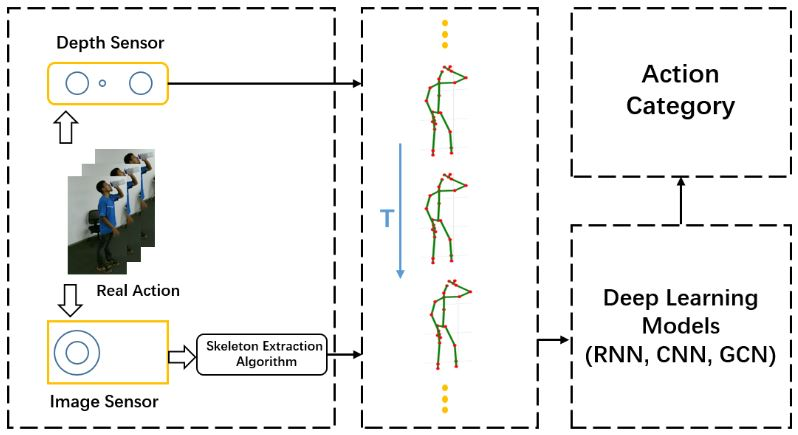
\includegraphics[width=.8\linewidth]{img/skeletonPipeline.JPG}
	\caption{Example from \cite{ren2020survey} the general pipeline of skeleton-based action recognition using deep learning methods. In the beginning, the skeleton data was gathered in two ways: directly from depth sensors or through pose estimate techniques.  The skeleton will be fed into neural networks based on RNN, CNN, or GCN.  Finally, we get to the action category.}\label{fig:skeletonPipeline}
\end{figure}

\subsection{RNN-Based Methods}
Recurrent Neural Networks as ~\ref{fig:LSTMSkeleton}, have been widely adopted to capture temporal dependencies in skeleton sequences. Specifically, in \cite{zhang2018adding} the result of the prior time step is used as the input for the current time step to create a recursive connection inside an RNN structure. A novel approach to adding attentiveness to RNN neurons. The proposed method is a simple yet effective way to adaptively weight the input elements of an RNN block at each time step. Moreover, the proposed method reduces computational overhead compared to existing attention mechanisms and is flexible in adapting to different types of RNNs, such as LSTM or GRU. The proposed method called EleAtt-RNN block addresses the challenges of modeling complex sequential information with fixed-weight RNNs and the limitation of existing attention mechanisms that require additional parameters and computational overhead. However, The performance of various related methods (e.g., \cite{wu2014leveraging}, \cite{zhao2017two}) often was unable to achieve a competitive outcome due to the RNN-based architecture's poor spatial modeling capability.

\begin{figure}
	\centering
	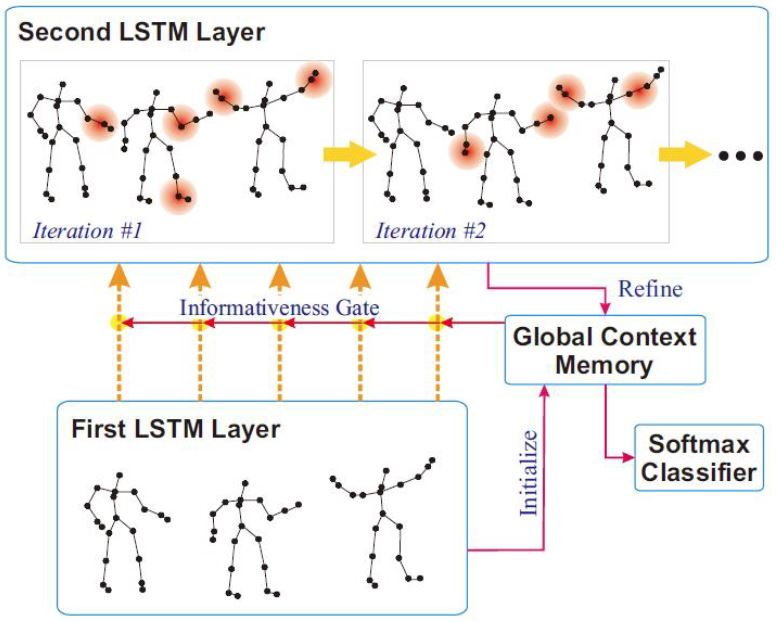
\includegraphics[width=.6\linewidth]{img/LSTMSkeleton.JPG}
	\caption{Example of RNN pipeline from \cite{Liu_2018} demonstrates how each joint has a distinct level of necessity for a specific skeleton action.}\label{fig:LSTMSkeleton}
\end{figure}
 
\subsection{CNN-Based Methods}
Convolutional Neural Networks have been extended to handle skeleton data by treating joint coordinates as image-like representations. Unlike RNNs, which explicitly model temporal dependencies in sequences, CNNs were originally designed for image-based tasks and lacked inherent temporal modeling capabilities. However, researchers have creatively adapted CNN architectures to effectively handle skeleton data by exploiting skeleton sequence data from vector sequence to pseudo-image. The main benefit of CNN-based methods over RNNs lies in their ability to efficiently capture spatial relationships among joints. CNNs are adept at learning hierarchical representations from image data, effectively recognizing local patterns and capturing spatial dependencies. This property aligns well with the inherent structural information in skeleton data, where each joint's position relies on its relationship with neighboring joints. This spatial awareness allows CNNs to learn discriminative features from skeleton sequences and recognize actions based on joint configurations and their temporal dynamics.\cite{ding2017investigation} investigate encoding richer spatial features into texture color images or 2D pseudo-images for 3D human action recognition using a CNN-based approach. Each type of feature is encoded into images in two or more ways to further explore the spatio-temporal information. The proposed method consists of five main components: spatial feature extraction from input skeleton sequences, key feature selection, texture color image encoding from key features, CNN model training based on images, and score fusion. One of the challenges that this paper solves is the limitation of using only joint positions for skeleton-based action recognition. By encoding richer spatial features into texture color images, the proposed method is able to capture more detailed information about the motion and shape of the human body, leading to improved recognition accuracy.

Still, this type of approach is a little complex and also misses out on crucial data throughout the mapping process. To address this problem, \cite{li2017skeleton} propose a translation-scale invariant transformation approach to map 3D skeleton videos to color images with enhanced temporal frequency adjustment capabilities, using a multi-scale deep CNN. Each frame's human skeleton joints were initially divided into five main sections in accordance with human physical structure, and those sections were then transferred to 2D form. With this technique, the skeleton picture is created using both spatial and temporal information. In addition, they employ various data augmentation methods specifically designed for 3D skeleton data to improve the generalization ability of the network. Still, even though the way it performed was enhanced, there is still no reason for treating the skeleton's joints as isolated entities since in the real world, our bodies are highly interconnected. For instance, when walking, other body parts like the hands and the hip should also be taken into consideration in addition to the joints directly within the legs. The shape-motion representation derived from geometric algebra was presented by \cite{li2019learning}, addressed the significance of both joints and bones, and completely utilized the data offered by the skeleton sequence, as shown in ~\ref{fig:3DCNN_shapeMotion}.

\begin{figure}
	\centering
	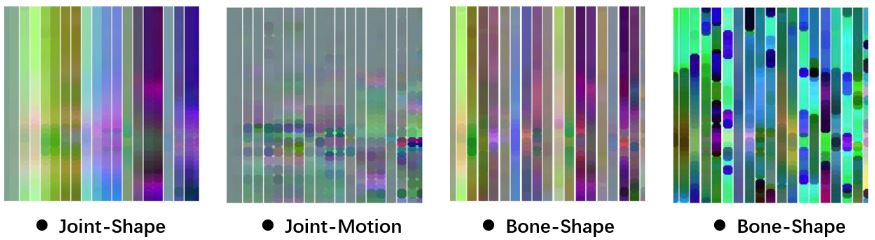
\includegraphics[width=.7\linewidth]{img/3DCNN_shapeMotion.JPG}
	\caption{Demonstration of the shape-motion representation given out by \cite{li2019learning}.}\label{fig:3DCNN_shapeMotion}
\end{figure}

 In this context, each skeleton joint is treated as a row and column in an image, and temporal dynamics are encoded through convolutional operations. However, this approach limits the consideration of co-occurrence features among all joints, as only neighboring joints within the convolutional kernel are considered. As a result, crucial correlations that may be related to the entire skeleton structure might be overlooked, preventing CNNs from learning comprehensive and useful features. Researchers have attempted to tackle this issue and enhance the representation capabilities of CNNs for skeleton data. \cite{li2018co} proposed an innovative end-to-end framework that employs a hierarchical approach to aggregate different levels of contextual information gradually. Firstly, point-level information is independently encoded, and then it is assembled into a semantic representation in both the temporal and spatial domains. By learning co-occurrence features with this approach, the model gains a more comprehensive understanding of the relationships among skeleton joints, improving its ability to recognize complex actions. Other challenges persist in these methods as the size and speed of the model, which can hinder real-time applications and require substantial computational resources. \cite{yang2019make} delves into techniques for optimizing CNN architectures to achieve more efficient models without sacrificing accuracy. Moreover, CNN-based methods can be sensitive to occlusions, viewpoint changes, and other variations in action sequences. Researchers have explored solutions to improve the robustness of CNNs in handling these challenges. For instance, \cite{liu2017enhanced} investigates methods to enhance skeleton visualization for improved action recognition under varying viewpoints.

 In summary, while CNN-based methods have shown promising results in skeleton action recognition, they face unique challenges related to co-occurrence feature learning, model efficiency, and robustness. Researchers continue to explore novel architectures, aggregation techniques, and optimization strategies to address these issues and advance the capabilities of CNNs in effectively recognizing actions from skeleton data. As an ongoing open problem, further investigation and innovation in CNN-based techniques hold the potential to unlock even more robust and accurate skeleton action recognition models.
 
\subsection{GCN-Based Methods}
The inherent topological graph structure of human 3D-skeleton data sets it apart from traditional sequence vectors or pseudo-images typically used in RNN-based or CNN-based methods. In recent years, Graph Convolutional Networks (GCNs) have emerged as a popular choice for effectively representing and processing graph-structured data, including skeleton graphs. There are two main types of graph-related neural networks: Graph and Recurrent Neural Networks (GNN) and Graph and Convolutional Neural Networks (GCN), research was focused primarily on the latter. The application of GCNs to skeleton-based action recognition has shown promising results, displaying convincing performance on various benchmarks. Unlike simply encoding skeleton sequences into sequence vectors or 2D grids, GCNs offer the ability to fully express dependencies between correlated joints. These networks, as a generalization of CNNs, can be applied to arbitrary structures, making them suitable for modeling the complex connectivity in skeleton graphs.

One notable model that utilizes GCNs for skeleton-based action recognition is the "Spatial Temporal Graph Convolutional Networks" (ST-GCN) presented in \cite{yan2018spatial}. This novel approach constructs a spatial-temporal graph with joints as graph vertices and natural connectivities in both human body structures and time as graph edges. The ST-GCN model learns higher-level feature maps on the graph and subsequently classifies them using a standard Softmax classifier to predict the corresponding action category. Since the introduction of ST-GCN, the use of GCNs for skeleton-based action recognition has garnered significant attention, leading to various related works. Researchers have focused on efficiently utilizing skeleton data and exploring richer dependencies among joints. For instance, "Actional-Structural Graph Convolutional Networks" (AS-GCN), proposed in \cite{li2019actional}, not only recognizes a person's action but also employs a multi-task learning strategy to predict the subject's next possible pose. The constructed graph in AS-GCN captures richer dependencies through two modules: Actional Links and Structural Links, as shown in ~\ref{fig:GCN_method}.

However, the most common concern across GCN-based action recognition studies remains data-driven, aiming to uncover the latent information hidden within 3D skeleton sequence data. The challenge lies in acquiring and transforming the skeleton data into a graph representation while preserving its temporal-spatial coupling and considering the connections among joints and bones. Another significant concern and challenge in GCN-based action recognition lies in effectively handling temporal dependencies within skeleton sequences. While GCNs are adept at capturing spatial relationships among joints in a single frame, they may struggle to explicitly model long-range temporal dependencies that span multiple frames. This limitation can impact the model's ability to recognize complex actions that involve intricate temporal dynamics.

\begin{figure}
	\centering
	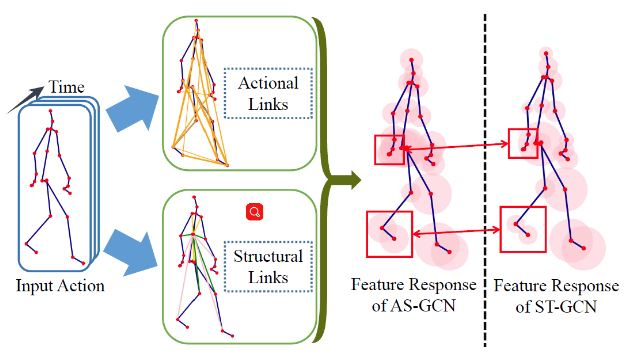
\includegraphics[width=.7\linewidth]{img/GCN_method.JPG}
	\caption{Demonstration of the feature learning in AS-GCN \cite{li2019actional} with generalized skeleton graphs. The actional links and structural links capture dependencies between joints. Compared to ST-GCN, AS-GCN obtains responses on collaborative moving joints (redboxes).}\label{fig:GCN_method}
\end{figure}


\subsection{Self-Attention Mechanism-Based Methods}
The revolutionary Transformer model, as introduced in \cite{vaswani2017attention} has made significant strides in natural language processing and has since been adopted in various domains, including computer vision. At the core of the Transformer's success lies its self-attention mechanism, which allows it to learn relationships between elements within a sequence effectively. This key feature enables Transformers to handle long sequences, a limitation that GCNs face as we mentioned before, and also traditional LSTM and RNN networks struggle with. The multi-headed self-attention mechanism further boosts efficiency by processing sequences in parallel, departing from the recursive word-by-word approach of LSTM and RNN networks. The advantages of self-attention have paved the way for its application in computer vision tasks, such as image classification and recognition, as demonstrated in \cite{wu2021cvt}. This work combines the strengths of CNNs and self-attention to model both local and global dependencies in images, resulting in improved performance for image classification tasks. Similarly, in \cite{bertasius2021space} self-attention was applied to learn spatio-temporal features from sequences of frame-level patches for video action recognition. The method effectively captured both spatial and temporal relationships, enhancing the model's ability to understand complex actions in videos.

Inspired by the success of Transformers and self-attention in computer vision, researchers have extended these principles to skeleton action recognition. In \cite{plizzari2021skeleton} the authors introduced a novel approach that utilizes self-attention instead of regular graph convolutions in both spatial and temporal dimensions. This extension of self-attention into the graph structure of skeleton data allowed the model to effectively capture dependencies between joints in space and time, leading to improved action recognition performance. By incorporating self-attention into the GCN framework, this method enables more comprehensive modeling of the complex interactions among skeleton joints, addressing the challenge of effectively capturing long-range temporal dependencies. Since distinct body components (such the arms and legs in "walking") between adjacent frames move simultaneously, the correlation of different joints across frames, which the previous Transformer-based approaches cannot capture, is particularly useful. The STTFormer is an approach in \cite{qiu2022spatio}, which is a novel spatio-temporal tuples transformer, where the skeleton sequence is broken up into multiple sections, and each portion has numerous consecutive frames that are encoded. The link between various joints' non-consecutive frames is then captured by a spatio-temporal tuples self-attention module (STTA). In order to improve the capacity to differentiate identical activities, a feature aggregation module (IFFA) was also included between non-adjacent frames. This model has shown better performance on benchmark datasets when compared to state-of-the-art methods. In this study, we will use ST-GCN, and the self-attention mechanism with the STTFormer model to investigate the capabilities of both techniques on different frameworks and learning strategies such as self-supervised learning which will discuss in the following section.

\section{Self-Supervised Learning}
Traditional supervised learning methods for computer vision tasks require large annotated datasets, which can be time-consuming and expensive to produce. Additionally, unsupervised learning methods lack guidance and may not generate meaningful representations. Self-Supervised Learning (SSL) offers a compelling solution to these challenges by leveraging unlabeled data to learn useful representations without the need for external annotations. Self-Supervised Learning is a branch of machine learning where a model learns to predict or reconstruct certain parts of its input data without explicit supervision. The model is trained to solve pretext tasks, which are constructed from the data itself, rather than relying on externally labeled datasets.

By employing pretext tasks, the model learns to capture meaningful features from the data, which can then be transferred to downstream tasks, as shown in ~\ref{fig:SSL_pipeline}. In supervised learning, the model is trained on labeled data with input-output pairs, whereas in unsupervised learning, the model aims to discover underlying patterns in unlabeled data. SSL falls between these two paradigms, utilizing unlabeled data and transforming it into labeled-like data by creating pretext tasks that serve as supervisory signals for training.



\subsection{SSL: Pretext Tasks}
Early research in SSL explored various pretext tasks to effectively exploit unlabeled data. A common approach involved training models to predict missing parts of an input image, such as inpainting or image completion tasks. By predicting masked-out regions, the model learned to understand contextual relationships within the image. Papers such as \cite{pathak2016context} and \cite{yu2018generative} delved into this area. In \cite{gidaris2018unsupervised} contributed to the development of another prevalent pretext task was image rotation, where the model learned to predict the rotation angle applied to an image. This task encouraged the model to capture semantic information and invariant features in different orientations. Recent advancements in SSL have explored novel approaches, including pretext tasks and contrastive learning methods. One notable research direction focuses on pretext tasks, where the model learns from multiple transformations of the same input data, such as jigsaw puzzles in \cite{noroozi2016unsupervised}, colorization \cite{larsson2016learning}. These pretext tasks offer diverse learning signals, leading to more robust feature representations. is a pioneering work in this area.

\begin{figure}
	\centering
	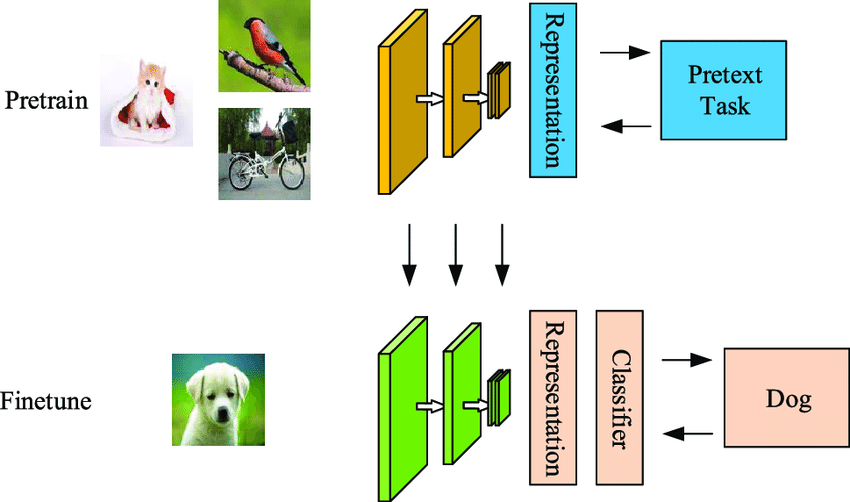
\includegraphics[width=.7\linewidth]{img/SSL_pipeline.png}
	\caption{The general pipeline for SSL from pre-training the model with a pretext task then transferring to a downstream task, source from \cite{v7labs2022ssl}.}\label{fig:SSL_pipeline}
\end{figure}


\subsection{SSL: Contrastive Learning}
On the other hand, contrastive learning has gained popularity, where the model is trained to pull similar instances closer in the embedding space while pushing dissimilar instances apart, as shown in ~\ref{fig:ContrastiveLearning}. This method enables the model to learn high-level feature representations that effectively capture the inherent structure of the data. One of the pioneering works in contrastive learning is (CPC) \cite{oord2018representation}. CPC formulates a pretext task where the model predicts future audio segments given past segments. The key insight behind CPC is to contrast the predictions of true future segments with other negative samples, forcing the model to learn representations that capture relevant information for future prediction. Papers such as \cite{he2020momentum} and \cite{chen2020simple} have significantly contributed to the advancements in contrastive learning. \cite{he2020momentum} leveraged momentum contrast to create a contrastive loss. The model uses a moving average of the model's weights, known as the momentum encoder, to generate a key representation for each data sample. The main encoder then generates a query representation, and the contrastive loss encourages the model to maximize agreement between the query and key representations for positive samples while minimizing agreement for negative samples.

One of the primary challenges in early contrastive learning methods was the choice of negative samples. In the CPC method, selecting negative samples from the same audio sequence resulted in the model learning trivial solutions. To overcome this, researchers introduced more sophisticated strategies to create informative negative samples, such as using samples from other data instances or different time steps. Additionally, contrastive learning was computationally demanding as it required comparing each positive sample with all possible negative samples. Early research explored techniques to speed up the process, such as using large memory banks for negative samples and employing batch normalization for efficiency.

Recent research as \cite{chen2020simple} introduced the SimCLR framework, which demonstrated the effectiveness of large-batch contrastive learning and data augmentation plays a critical role in defining effective predictive tasks. However, a limitation of SimCLR lies in its reliance on large batch sizes, which might not be practical for all hardware configurations. Another notable work is (SwAV) \cite{caron2020unsupervised}, which proposed a novel clustering-based approach for contrastive learning. While SwAV achieved impressive results, its success relies on having a large number of data samples, which might pose challenges for small-scale datasets.

In \cite{grill2020bootstrap}, the authors introduced (BYOL) an innovative approach to self-supervised learning that are negative-sample-free and not relying on negative pairs, which solves the issue of mining the relevant negative pairs and it doesn't need the explicit generation of negative sample pairs. In \cite{caron2021emerging} (DINO) they were inspired by (BYOL) and they proposed an asymmetric network based only on positive pairs to prevent feature collapse. This recent research achieved state-of-the-art results by leveraging an ensemble of neural networks to learn and bootstrap their own unsupervised representations.

\begin{figure}
	\centering
	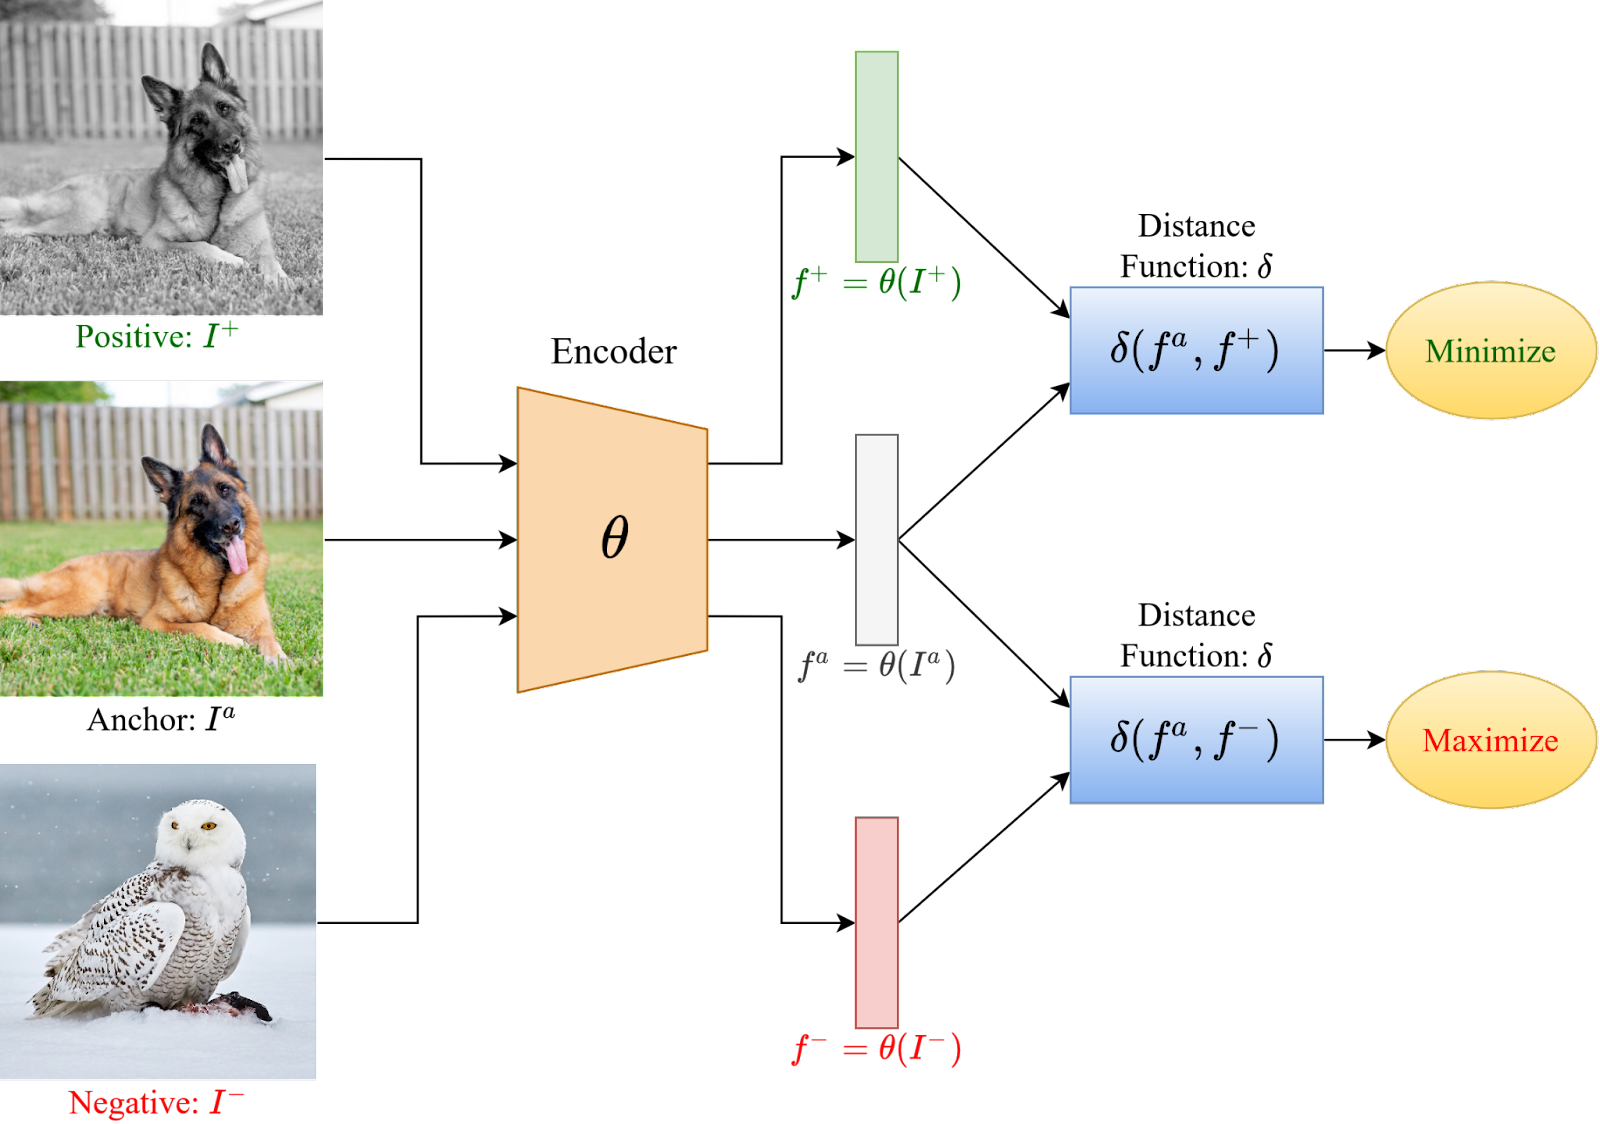
\includegraphics[width=.6\linewidth]{img/ContrastiveLearning.png}
	\caption{Demonstration in \cite{v7labs2022contrastive} of contrastive learning by minimizing the similarity function between the anchor and the positive sample, and maximizing the distance between the anchor and the negative sample.}\label{fig:ContrastiveLearning}
\end{figure}


\subsection{Evaluating SSL models}

Evaluating the performance of SSL methods requires careful consideration due to the absence of traditional supervised labels. Researchers have devised various evaluation techniques to assess the quality of learned representations and the effectiveness of pretext tasks in capturing meaningful features.

One common evaluation metric in SSL is the "linear evaluation protocol," where the learned representations are fine-tuned on downstream tasks using simple linear classifiers. By using linear classifiers, researchers can measure the quality of the learned features without introducing additional complexity from complex classifiers or fine-tuning the entire model. The performance of these linear classifiers on downstream tasks serves as a proxy for evaluating the generalization capability of the learned representations. Another crucial aspect of SSL evaluation involves assessing how well the learned representations transfer to downstream tasks. SSL models aim to capture high-level features, which should be transferable to various computer vision tasks. Transfer learning to tasks such as image classification, object detection, and semantic segmentation can be employed to evaluate the effectiveness of learned representations in real-world applications.

A key evaluation consideration in SSL is the comparison between fine-tuning the entire model and using a linear classifier on top of the frozen backbone. Fine-tuning the entire model on downstream tasks allows for further adaptation to specific task domains, potentially achieving higher task-specific performance. However, fine-tuning may lead to overfitting or require a substantial amount of labeled data, which defeats the purpose of SSL. On the other hand, using linear classifiers on top of the frozen SSL backbone is computationally efficient and avoids overfitting issues. This approach allows researchers to evaluate the transferability of learned representations without requiring additional labeled data for fine-tuning. Although fine-tuning may yield better results on task-specific metrics, linear evaluation provides valuable insights into the generalization capabilities of the SSL model across different tasks.

The success of SSL lies in its ability to learn generic feature representations, which can be transferred to a wide range of downstream computer vision tasks. Some common downstream tasks include:

\begin{itemize}
	\item \textbf{Classification:} Evaluating the SSL model's ability to classify objects on the learned features. This is one of the most common and widely used downstream tasks for SSL evaluation.

	\item \textbf{Object Detection:} Assessing the performance of the SSL model on detecting and localizing objects within an image. This task evaluates the representations' capacity to capture object-level information.

 	\item \textbf{Semantic Segmentation:} Evaluating the model's ability to segment an image into different object categories or regions. This task tests the model's capability to understand spatial relationships within an image.

  	\item \textbf{Action Recognition:} Assessing the model's performance on recognizing and classifying actions from video sequences. This task examines the representation's ability to capture temporal dynamics.

   	\item \textbf{Domain Adaptation:} Evaluating the transferability of learned representations across different domains or datasets. This task is critical for assessing SSL models' generalization across various real-world scenarios.
     
\end{itemize}

In conclusion, Self-Supervised Learning presents a compelling alternative to traditional supervised and unsupervised learning approaches, harnessing the potential of unlabeled data to learn informative representations. Through pretext tasks and contrastive learning, SSL has demonstrated remarkable success in solving computer vision tasks and continues to be an active area of research in the field of machine learning.



\section{Self-supervised skeleton-based action recognition}
Self-supervised learning has emerged as a promising approach for learning informative representations from unlabeled data in the context of skeleton-based action recognition. Researchers have explored various self-supervised techniques to leverage the temporal dynamics and spatial information present in skeleton data. In the paper \cite{zheng2018unsupervised} the authors proposed a method based on a recurrent encoder-decoder GAN to reconstruct the input skeleton sequence. By learning to reconstruct the input sequence, the model can capture long-term temporal dynamics and subtle motion patterns essential for action recognition. Building on the ideas of reconstruction, the research (Predict\&Cluster) in \cite{su2020predict} introduced a decoder to improve the representation ability of the encoder. The method leverages both prediction and clustering to encourage the model to learn more discriminative and compact representations.

In \cite{lin2020ms2l} authors proposed (MS2L) a multi-task framework, including motion prediction and jigsaw puzzle tasks, to enhance the model's understanding of motion and spatial relationships among joints. By jointly solving multiple tasks, the model can capture richer information from the skeleton sequences. (AS-CAL) was introduced in \cite{rao2021augmented} as an approach that utilizes momentum LSTM to regularize the feature space. Along with various skeleton augmentation strategies, this method aims to enhance the model's robustness and generalization capability. In \cite{li20213d} proposed SkeletonCLR, which applies a memory bank to store negative samples and employs a cross-view knowledge mining strategy. By leveraging the memory bank and cross-view consistency, the model can capture more comprehensive and discriminative representations. In order to add movement patterns and compel the encoder to acquire broader representations, (AimCLR)  proposes to make extensive use of augmentation.  The amount of redundant information within the spatial joints and temporal frames, which might increase the strength of 3D visual representation and are crucial for downstream tasks, has not been taken into account. These contrastive learning approaches, on the other hand, significantly rely on powerful data augmentation procedures.

The Partial Spatio-Temporal Learning (PSTL) is a recent research published in 2023 in \cite{zhou2023self} proposed to address the limitations of existing methods in skeleton-based action recognition. While current approaches focus on a global perspective to discriminate different skeletons, PSTL aims to leverage the local relationship between various skeleton joints and video frames, which is crucial for real-world applications. PSTL adopts a unique spatio-temporal masking strategy to construct partial skeleton sequences, allowing the model to focus on specific regions of interest. The framework utilizes a negative-sample-free triplet stream structure, comprising an anchor stream without any masking, a spatial masking stream with Central Spatial Masking (CSM), and a temporal masking stream with Motion Attention Temporal Masking (MATM). These innovative components facilitate the exploitation of local dependencies and cues within the skeleton sequences, ultimately leading to improved action recognition performance. As part of this research, we will further investigate the efficacy of PSTL with different settings and diverse datasets to comprehensively validate its potential in advancing skeleton-based action recognition.